\section{Эксперимент}
\subsection{Часть}
\begin{equation}
    NH_4Cl + NaOH \to NaCl + H_2O + NH_3 \uparrow
\end{equation}

Классический пример реакции нейтрализации, кислота реагирует
с основанием в результае образуется раствор соли. Аммиак 
являющийся основанием, испаряется в следствии чего лакмусовая 
бумага меняет свой цвет. В моем случае окарс сответстовал 
$pH \approx 6-7$.


%Фото у Некиты

\subsection{Часть}
\begin{equation}
    NH_4Cl \xrightarrow{Heat} NH_3\uparrow + HCl\uparrow
\end{equation}
Реакция эндотермическая, но в резульмтате хлорид амония 
разлогается на летучие газы $NH_3 \land HCl$.

\begin{figure}[h]
    \centering
    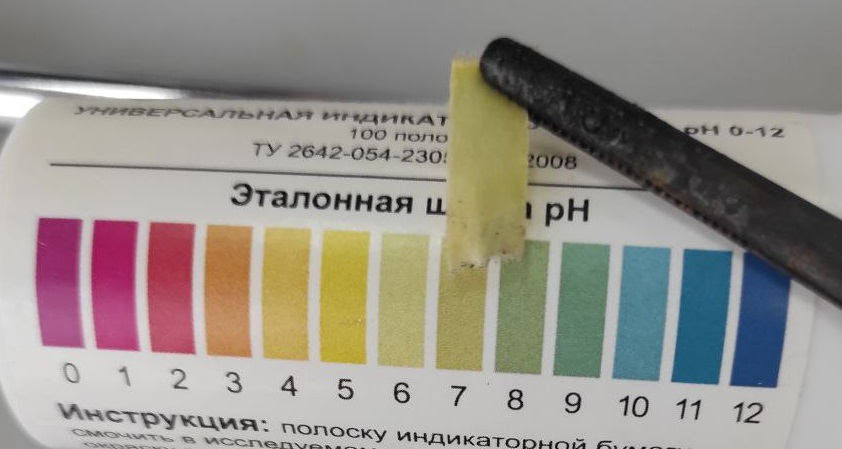
\includegraphics[width=1\linewidth]{Ex_4/2.jpg}
     \caption{Степень $pH$}
    \label{ex_4_2}
\end{figure}




